\documentclass{article}
\usepackage[colorlinks=true,linkcolor=blue,citecolor=blue]{hyperref}
\usepackage{siunitx}
\usepackage{amssymb}
\usepackage{amsmath}
\usepackage{bm}
\usepackage{subcaption}
\usepackage{cancel}
\usepackage{graphicx}
\usepackage{gensymb}
\graphicspath{{Day8NotesPics/}}
\author{Mann, J}
\title{Day 8 Notes}
\date{September 22, 2015}
\renewcommand{\d}[0]{\mathrm{d}}
\renewcommand{\deg}[0]{\degree}
\newcommand{\note}[1]{\vspace{\parsep}\textbf{\textit{Note: }}#1\\\\}
\newcommand{\matr}[1]{\bm{#1}}
\newcommand{\diag}[1]{\bcancel{#1}}
\newcommand{\dOne}[2]{\frac{\d #1}{\d #2}}
\newcommand{\pOne}[2]{\frac{\partial #1}{\partial #2}}
\newcommand{\dTwo}[3]{\frac{\d^2 #1}{\d #2^2}}
\newcommand{\pTwo}[3]{\frac{\partial^2 #1}{\partial #2^2}}
\newenvironment{aside}{\hrulefill\begin{flushright}}{\\\hrulefill\end{flushright}}

\begin{document}
\maketitle
\begin{section}{Introduction}
%	\begin{enumerate}
%		\item Taking numerical derivatives
%		\item Inversion of the virial isotherm
%		\item Consider various fitting functions for the analysis of liquid/vapor and liquid/liquid systems. Also the liquid or vapor/solid interface
%		\item The measurement of surface tension
%	\end{enumerate}
	\tableofcontents
	Next time 2-D crystal structures
\end{section}
\begin{section}{The derivative of experimental data}
Raw isotherm made with a Langmuir monolayer, as you compress it, thre is a region where they do a phase transition . Then you get a 2D liquid state, then a 2D solid (which may be highly structured)
What's useful here is to take $\dOne{\pi}{A}$ and multiply it by $-A$, which gives you an analog in two dimensions of the inverse of the compressibility.

A numerical derivative will be nonsense if you don't do it right. Try fitting it to a model, then take a derivative with respect to the fitted model. It still won't be perfect, however.
\end{section}
\begin{section}{\href{https://blackboard.case.edu/courses/1/eche464_jam12/content/_1224783_1/processingvirialdata2.pdf}{See notes online for inverting the virial isotherm}}
\end{section}
\begin{section}{Tensiometers}
	A well-known manufacturer is Kr\"uss

	\begin{subsection}{Classical Method: Capillary Rise}

		\begin{figure}[h]
			\centering
			\begin{subfigure}[t]{0.3\textwidth}
			\centering
				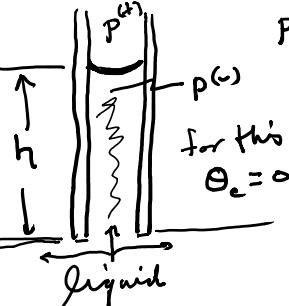
\includegraphics[height=100pt]{capillaryRise1}
						\caption{A typical capillary rise setup}
			\end{subfigure}
			\begin{subfigure}[t]{0.3\textwidth}
			\centering
				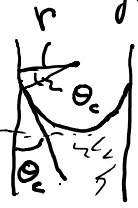
\includegraphics[height=60pt]{capillaryRise2}
						\caption{the contact angle $\theta_c$ is the slope of the line made tangent to the surface at the interface.}
			\end{subfigure}
			\begin{subfigure}[t]{0.3\textwidth}
			\centering
				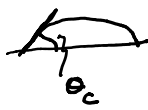
\includegraphics[height=20pt]{capillaryRise3}
						\caption{A closeup of $\theta_c$}
			\end{subfigure}
								\label{fig:capillary}
		\end{figure}
	\begin{align*}
		P^{(+)}&>P^{(-)}\\
		\Delta P &= \rho g h = \gamma \left(\frac{1}{R_1}+\frac{1}{R_2}\right) = \frac{\gamma}{R}\\
		\frac{r}{R} &= \cos{(\theta_c)}
	\end{align*}
	\begin{figure}[b]
		\centering
		\begin{subfigure}[t]{0.3\textwidth}
			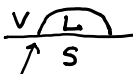
\includegraphics[height=40pt]{3phasecontactside}
			\caption{Side view of the 3 phase contact line}
		\end{subfigure}
		\begin{subfigure}[t]{0.3\textwidth}
			\centering
			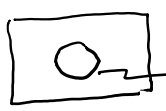
\includegraphics[height=40pt]{3phasecontacttop}
			\caption{Top view}
		\end{subfigure}
		\caption{The three phase contact line. The contact angle is the angle through the fluid from the surface. We will have quite a bit to say about contact angles later. }
		\label{fig:threephase}
	\end{figure}
	$r$ is the radius of the capillary, $R$ is the radius of the spherical cap. Capillaries are of glass with ``high-precision'' bores; $r$ must be uniform.
	Since $R_1=R_2$ when in a spherical cap, the capillary rise, $h$, is determined by:
	\begin{align*}
		\Delta\rho = \rho g h = \frac{2\gamma}{R}\\
		\frac{r}{R}=\cos{(\theta_c)}
	\end{align*}
	so that when $\theta_c = 0$,
	\begin{align*}
		\frac{\rho g h r}{2} = \gamma
	\end{align*}
	You will see that a ``capillary constant'' $a^2$ is defined as 
	\begin{align*}
		a^2 &= \frac{2\gamma}{\rho g} = h R\\
 		a^2 &[=] (\text{length})^2
	\end{align*}
	If $r$, the capillary radius, is too large, then the spherical cap is distorted by gravity. There would no longer be a single value of $R$.

	
We now define a new dimensionless variable, the bond number, $B_0$, which is a ratio between the force of gravity and the force of surface tension.
\begin{align*}
	B_0 &= \frac{\Delta \rho g r^2}{\gamma}\\
	\Delta\rho &= \text{Density jump}\\
	B_0 &<< 1 \text{ then the cap is spherical}\\
	r &>\text{ 2mm then the cap flattens, which is bad.}
\end{align*}
The rule is that $r$ should be small enough that $B_0 << 1$ for the interface to obey $r=R$ for $\theta_c = 0$.

There are experiments in which you want the confined interface to be flat. There are two ways to accomplish this:
\begin{figure}[h]
	\centering
	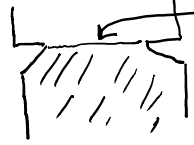
\includegraphics[height=40pt]{sharpInterface}
	\caption{An example of a small tube with a flat interface. This can be made optically flat by controlling the liquid level.}
	\label{fig:sharpInterface}
\end{figure}
\begin{enumerate}
	\item The surface could be treated with something to make the contact angle $90^\circ$. This can be hard to do.
	\item ``Pinning'' might work. This is a process where you put in a sharp lip (as sharp as you can make it - machining metal cell for example), then fill with fluid. Right at the lip, you will get the fluid to stop at the sharp point. Then you add more until the surface is level. See Figure~\ref{fig:sharpInterface}

\end{enumerate}
Geometric Methods for measuring $\gamma$ include
	capillary rise,
	pendant/bubble sessile drop, and
	captive bubble spinning drop
\end{subsection}
\begin{subsection}{Axisymmetric Drop Shape Methodology}

	\begin{figure}[h]
		\centering
		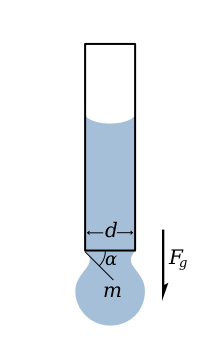
\includegraphics[height=100pt]{pendantDrop}
		\caption{Pendant drop test. You would take a picture with some diffuse light source so that the image looked something like this. Diagram by Urocyon and LightYear at en.wikipedia} 
		\label{fig:pendant drop}
	\end{figure}
	You can use a drop of liquid, with good illumination, such as one coming out of a narrow channel. A photographic record is needed, then you get an image of the drop shape, such as Figure~\ref{fig:pendant drop}. 

	Then, locating pixels in the 2D space of the image produces a data set
	\begin{align*}
		\text{DropTrace}:=\begin{cases}x = x(s)\\y = y(s)\end{cases}
	\end{align*}
	This data set provides the input to solve 
	\begin{align*}
		[\hat{n}\cdot\matr{P}\cdot\hat{n}] = 2\gamma H
	\end{align*} 
	for $\gamma$. Programs have been written for this analysis. See A.W. Neumann
	for drops formed at capillaries to do a number of things. You can get dynamics of adsorption to the surface by pulling the drop up and down. You can also do the inverse of this experiment, and measure the surface tension between the liquid and the vapor, including in situations with very high temperatures. This could be used for example with liquid iron.
\end{subsection}
\begin{subsection}{Sessile Drop Method}

	\begin{figure}[h]
		\centering
		\begin{subfigure}[b]{0.3\textwidth}
			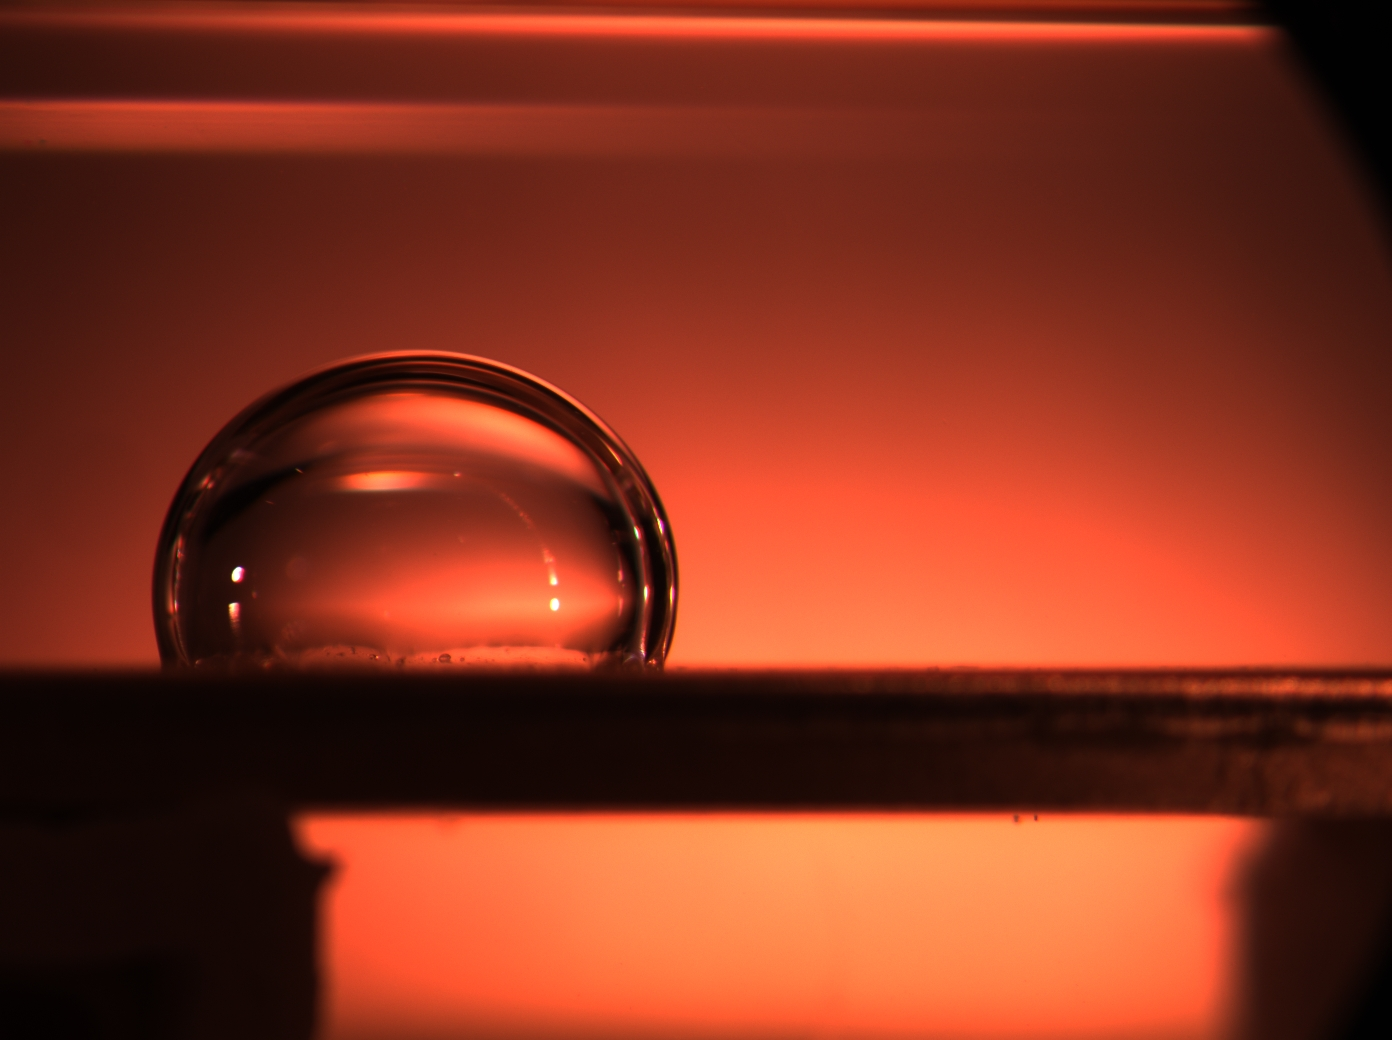
\includegraphics[height=100pt]{Water_droplet_in_oil_on_brass_surface}
			\caption{brass surface}
		\end{subfigure}
	\begin{subfigure}[b]{0.3\textwidth}
		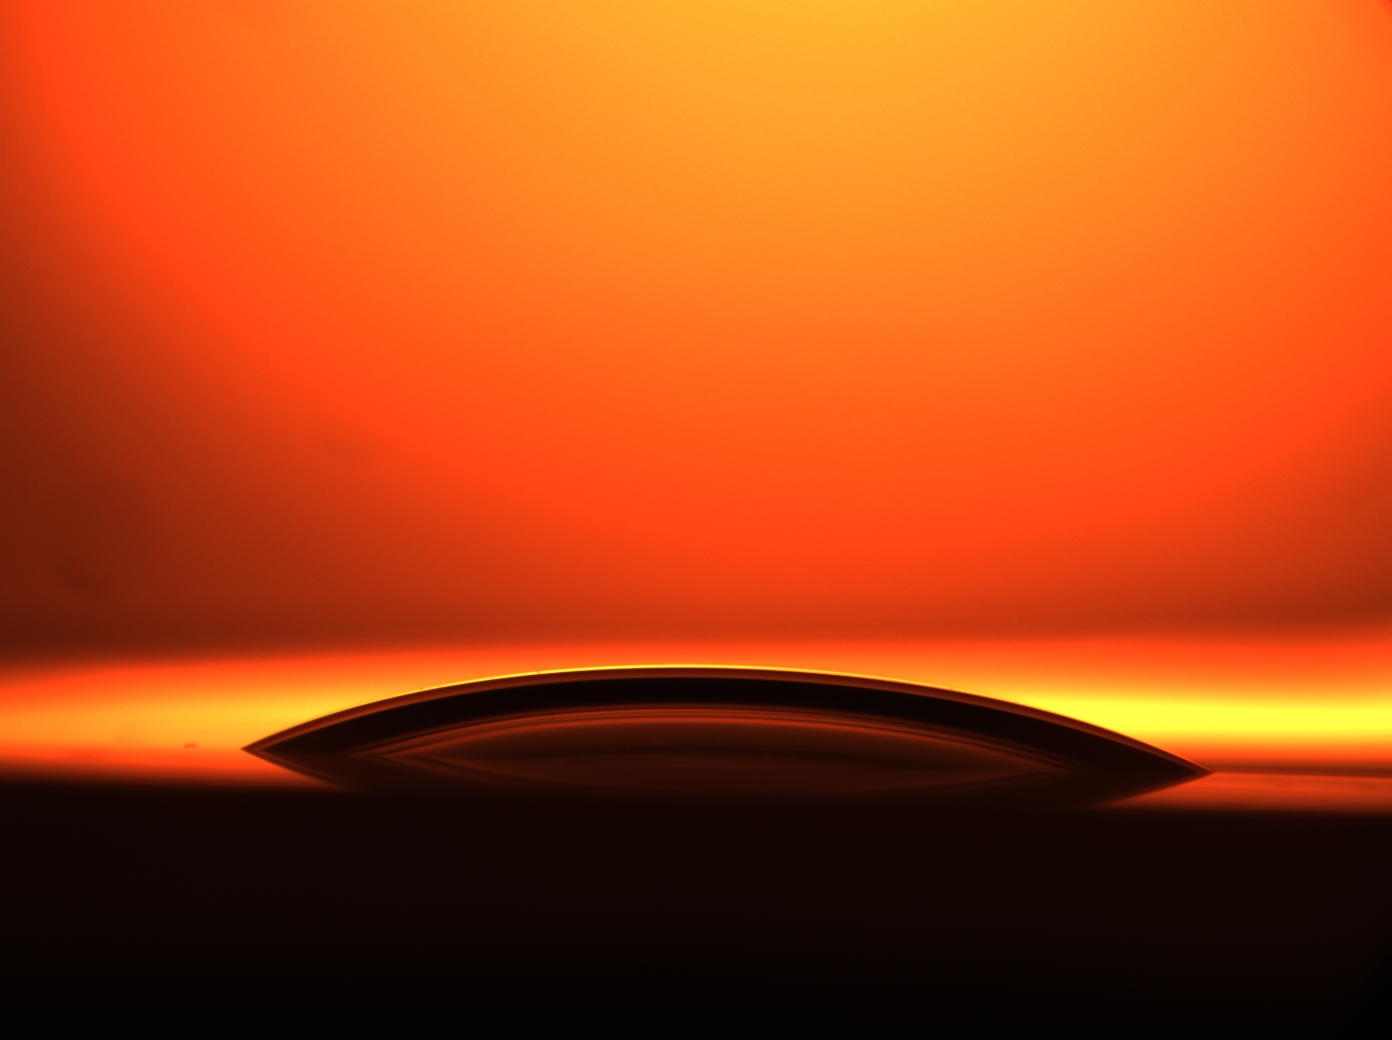
\includegraphics[height=100pt]{Water_droplet_in_oil_on_glass_surface}
		\caption{glass surface}
	\end{subfigure}
	\caption{Sessile drop pictures of water in oil on different surfaces. Photos by \href{https://commons.wikimedia.org/wiki/File:Water\_droplet\_in\_oil\_on\_brass\_surface.JPG}{Guro Aspenes}}
	\end{figure}
	This is a drop that is on a surface. You need to use the Laplace equation to get the surface tension and the contact angle of the fluid. The advantage of the imaging systems is that it's non-invasive. 
\end{subsection}
\begin{subsection}{Du N\"uoy Tensiometer}
	\begin{figure}[h]
		\centering
		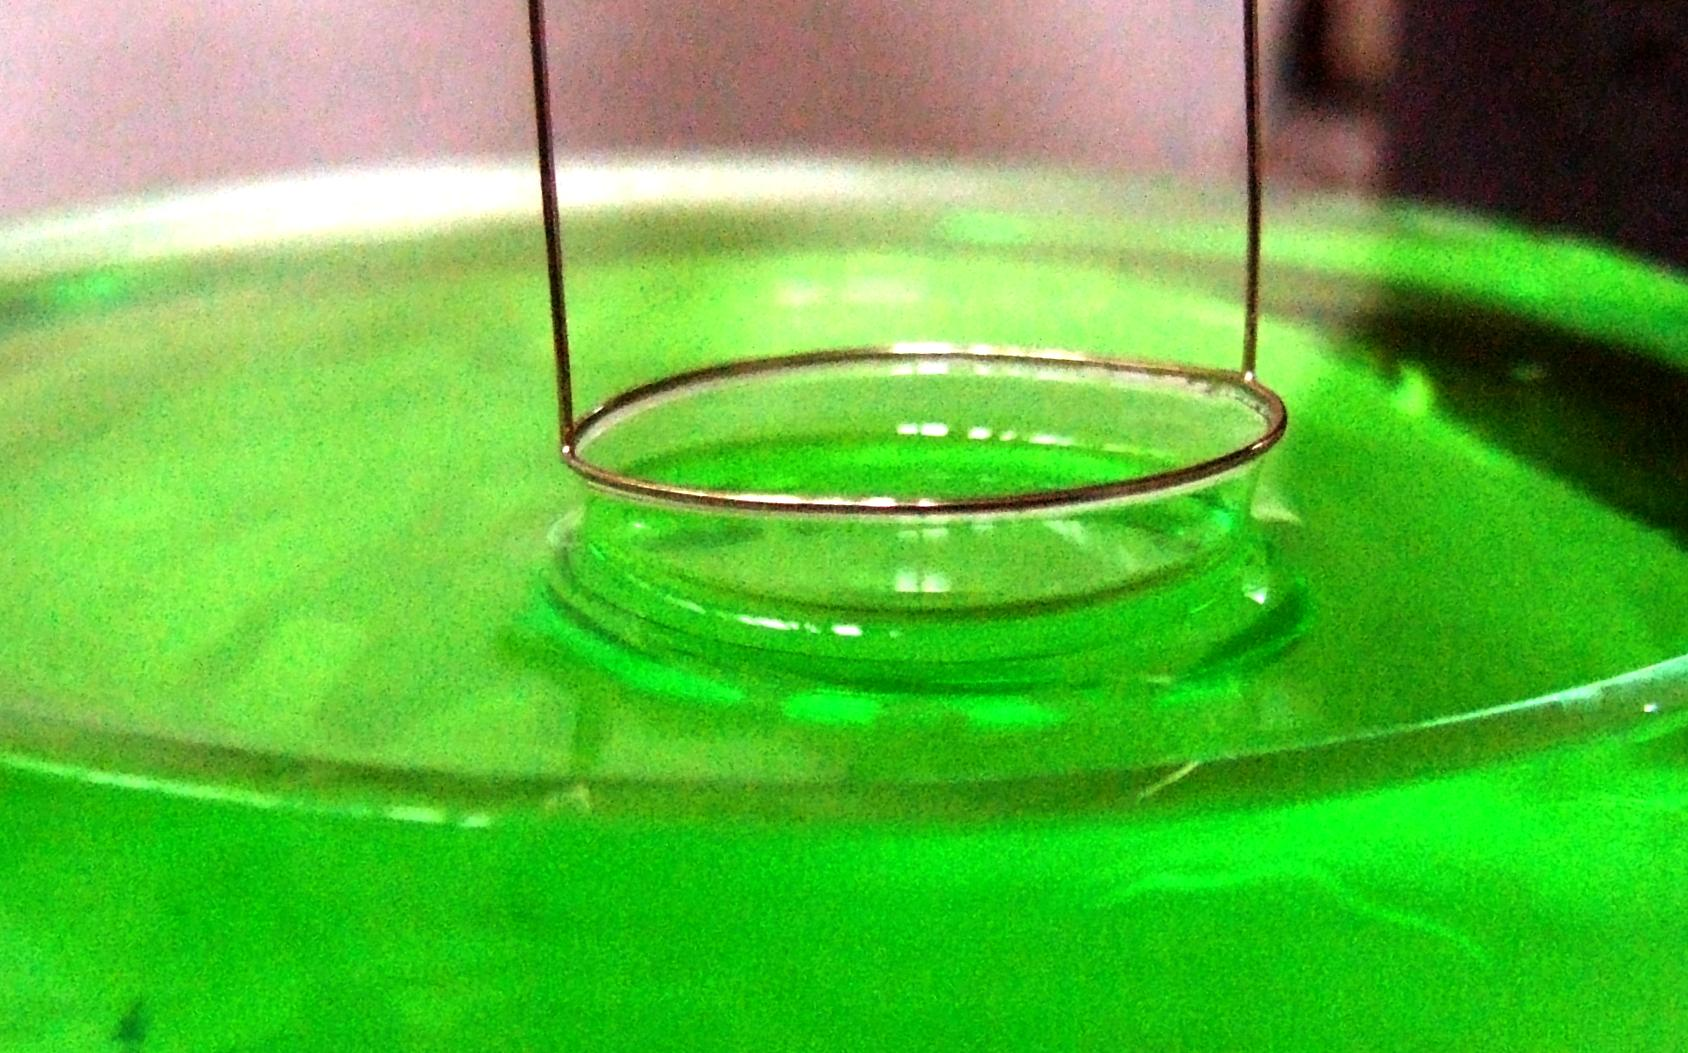
\includegraphics[height=100pt]{dunuoyring}
		\caption{A Du N\"uoy Ring Tensiometer. Photograph by Tibor Dubniczky}
		\label{fig:dunuoy}
	\end{figure}
	Measure the force necessary to detach the ring from the liquid.
	\begin{align*}
		\vec{F}_\text{necessary} = \frac{4\pi R}{F_c}
	\end{align*} where $F_c$ is a correction factor

	You can measure to a precision of parts per 100-parts per 1,000. Very precise. The problem is that you need a correction factor, which can amount to 10-15\% of the force. It depends on the radius of the wire. Folks in the 1930's worked out these correction factors, but they are not trivial, and without them the accuracy can be off by 20\% or more. With the proper correction factor, you can reach about results within about 1-2mN/m of the expected value. This is a fast, easy measurement that is popular in industry. You really just need to clean the ring before it can be used. A common method of doing this is by firing, since the ring is made of platinum. I \underline{really prefer} the plate method

	Again, this method is precise, but not accurate.
\end{subsection}
\begin{subsection}{Wilhemy Plate}
	\begin{figure}[h]
		\centering
		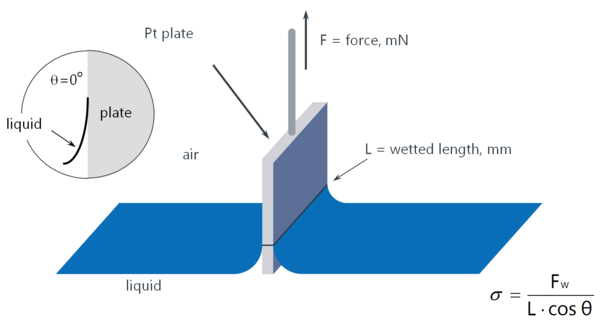
\includegraphics[height=100pt]{Wilhelmy_plate}
		\caption{A diagram of a Wilhelmy plate.	- \href{http://www.kruss.de/services/education-theory/glossary/wilhelmy-plate-method/}{Kr\"uss website}}
		\label{fig:wilhelmy}
	\end{figure}

You need a plate, 1-2cm, and a balance to measure the force. The plate is often made out of roughened platinum (expensive, but Pt is inert). Then bring the solution up so that it just touches the bottom of the Pt plate. See Figure \ref{fig:wilhelmy}
, you need zero contact angle. Again, with Pt, you need to make sure it is contaminant free. Getting it cherry red in a bunsen burner should work fine to accomplish this.  The plate is thin so that the perimeter, $p$ is
\begin{align*}
	2l+F_\text{thickness}
\end{align*}
where $F_\text{thickness}$ is a correction factor that is usually not required. The length $l$ is about 2cm or so. If the liquid is brought up carefully to where it is just touching the plate, the force can be measured with good precision and accuracy.
\begin{align*}
	F_\text{observed} = \gamma P - F_\text{bouyancy}
\end{align*}
where $P$ is the wetted perimeter and the experiment can be designed so that $F_\text{bouyancy}$ is ignorable. See how Kr\"uss does that.

The plate method can be used for a rod or a fiber. Moreover, given liquids of known $\gamma$, the plae or rod method can be used to measure the contact angle. 


\note{If a surface is rough, and the contact angle is less than $90^\circ$,  then $\theta_c$ will be decreased. If the smooth contact angle is greater than $90^\circ$, you will get a greater contact.}
The Wilhelmy Plate and Du N\"uoy Tensiometer are both contact methods.
\end{subsection}
\begin{subsection}{Maximum Bubble Pressure Method}
	\begin{figure}[h]
		\centering
		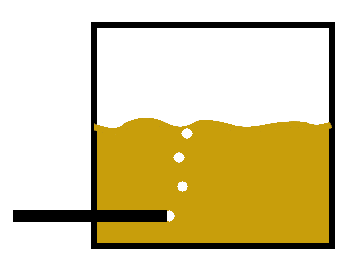
\includegraphics[height=100pt]{minimumPressure}
		\caption{Example maximum bubble pressure method. The cell is a closed cell half filled with some liquid (such as a molten salt). A capillary is brought in, and there is gas flow. Changing the pressure of the gas inside the capillary will allow you to measure the surface tension.}
		\label{fig:minimumPressure}
	\end{figure}
	Consider a liquid at (very) high temperature. The plate and ring methods will not work. However, the maximum bubble pressure method can be implemented.
	You change the pressure to grow the bubble - $P_\text{max}$ will be reached before the bubble detaches: 
	\begin{align*}
	P_\text{max} - P_\text{liq} = \frac{2\gamma}{r}
	\end{align*}
\end{subsection}
\end{section}
\newpage
\begin{section}{conclusion}
	For really careful, high precision, high accuracy - consider the drop imaging techniques. See A. W. Neumann's work. (Note that very low surface tensions ($10^{-2}$ mN/m for example) can be measured accurately.

	For convenience and reasonable accuracy I like the plate method - Kr\"uss sells a good instrument that is easy to use.

	I will lecture on surface light scattering spectroscopy at a later date.

The bottom line is that for fluids, we can do pretty well at measuring their surface tensions. For solids, though, it can be more difficult. Sometimes you can use spectroscopy if you are close enough to the liquid phase transition, but that doesn't always work very well. 

With solids, it is much easier to measure the mass of the material that adsorbs onto the interface

Some of you are familiar with the BET method for measuring the surface area per gram of packed powders.

Next time: Langmuir film that can form a solid in two dimensions.
3-D crystallography, extracting surface properties (ideal surface properties). Then talk about atoms on metal surfaces.
\end{section}
\end{document}
